\documentclass{article}



\usepackage{algorithm,algpseudocode}

\usepackage[margin=1in]{geometry}

\usepackage{enumerate}

\usepackage{graphicx}



\usepackage{amsfonts}

\def\R{{\mathbb R}}

\def\N{{\mathbb N}}



\title{In-Class Exercise 10}

\author{CSCI 432}

\date{28 October 2019}



\begin{document}

\maketitle



\noindent

Group Number:\\

Group members present today:



\section*{Max Flow / Min Cut}



\paragraph{Input:} We are given an acyclic graph $G=(V,E)$ with a weight function on the

edges $c \colon E \to \R$.  The weights are all non-negative and will be

referred to as \emph{capacities} of the edges.



\paragraph{Goal:} To find a flow of maximum value in the graph.  A \emph{flow}

is an assignment of weights to edges $\omega \colon E \to \R$ such that $0 \leq

\omega(e) \leq c(e)$ for all $e \in E$, and for all vertices $v \neq s,t$, flow

in is equal to flow out:

$$ \sum_{(x,v) \in E} \omega(x,v) = \sum_{(v,x) \in E} \omega(v,x) $$

The \emph{value of a flow} is equal to the flow out of

$s$ (and hence the flow into $t$): $val(\omega) = \sum_{(s,x) \in E}

\omega(s,x).$



The Ford-Fulkerson Algorithm is one algorithm that computes the max flow.

Examime the pseudocode and answer the questions below.



\begin{algorithm}

    {\bf Input:} $G=(V,E,c)$\\

    {\bf Output:} value of the maximum flow

    \begin{algorithmic}[1]

        \State Initialize weighted residual graph $R=(V'=V,E'=E,r=c)$

        \For{$e \in E$}

            \State Add edge $e^{-1}$ to $E'$ with weight $0$

        \EndFor

        \State $flow \gets 0$

        \While{$\exists$ path $p$ from $s$ to $t$ using positive edges of $R$}

            \State $\delta \gets \min_{e \in p} r(e)$

            \For{$e \in p$}

                \State $r(e) \gets r(e) - \delta$

                \State $r(e^{-1}) \gets r(e^{-1}) + \delta$

            \EndFor

            \State $flow \gets flow + \delta$

        \EndWhile

    \end{algorithmic}

\end{algorithm}



\begin{figure}

    \centering

    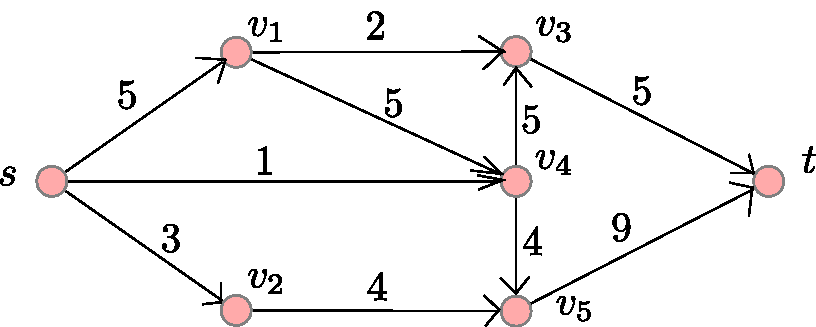
\includegraphics[height=2in]{figs/graph}

    \caption{A graph.  We wish to find the maximum flow from $s$ to

    $t$.}\label{fig:graph}

\end{figure}



\newpage

\begin{enumerate}

    \item Walk though the algorithm for Figure~\ref{fig:graph}.

    \item How can the algorithm be updated in order to return the actual flow

        $\omega$ in addition to the value of $\omega$?

    \item The number of times that the while loop executes is not unique.  Give

        an example of a graph and two different sequences of paths selected that

        result in the while loop executing a different number of times.

    \item How do we know that the while loop terminates?

    \item What is the loop invariant of the while loop?

\end{enumerate}



\end{document}
